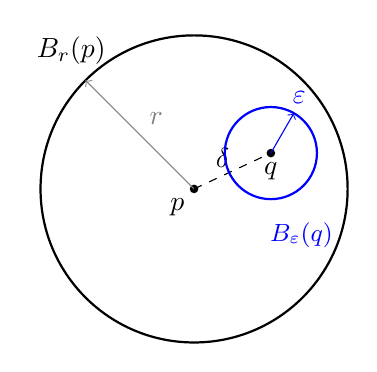
\begin{tikzpicture}[scale=1.3]
  \draw[thick] (0,0) circle (1.5);
  \fill (0,0) circle (1.2pt) node[below left] {$p$};
  \draw[->,gray] (0,0) -- (135:1.5) node[midway, above right] {$r$};
  \coordinate (q) at (0.75,0.35);
  \fill (q) circle (1.2pt) node[below] {$q$};
  \draw[dashed] (0,0) -- (q) node[midway, above left, inner sep=1pt] {$\delta$};
  \draw[blue, thick] (q) circle (0.45);
  \draw[->,blue] (q) -- ++(60:0.45) node[above, xshift=2pt] {$\varepsilon$};
  \node[blue] at (1.05,-0.45) {\small $B_\varepsilon(q)$};
  \node at (-1.2,1.35) {$B_r(p)$};
\end{tikzpicture}
